%!TEX root = informe.tex
\chapter{Análisis de Ciclo de Vida de un adoquín: evaluación del impacto ambiental}\label{cap:acv_evaluacion}

\section{Introducción}
La norma UNE–EN-ISO 14040:2006 \cite{iso14040} indica que ``la fase de EICV es para conocer y evaluar la magnitud y cuán significativos son los impactos potenciales ambientales de un sistema del producto a través de todo el ciclo de vida del producto''.

En esta etapa, se utilizan los datos recopilados en la fase de Inventario ICV vistos en el capítulo \ref{cap:acv_inventario} y se hace un enfoque relativo del impacto ambiental basado en la Unidad Funcional, convirtiendo los datos del ICV a unidades comunes, sumando posteriormente los resultados obtenidos dentro de la misma categoría de impacto, siguiendo la metodología explicada en la sección \ref{sec:metodologiaeicv}.

En este proyecto también se desarrollarán las etapas opcionales de normalización, agrupación y ponderación de los resultados.

Como se ha establecido la sección \ref{sec:categoriasimpactoseleccionadas}, para la elección de las categorías de impacto, el método ReCiPe recoge 18 categorías, de las cuales se ha seleccionado las más significativas mediante una previsualización de los resultados:
\begin{itemize}
  \item Cambio climático — Salud humana (CC[HH]).
  \item Toxicidad humana (HT).
  \item Formación de partículas (PMF).
  \item Cambio climático - Ecosistemas (CC[Ec]).
  \item Ocupación de tierras agrícolas (ALO).
  \item Transformación natural de la tierra (NLT).
  \item Agotamiento de recursos fósiles (FD).
\end{itemize}

Una vez introducidos los datos del inventario para todas las fases del ciclo de vida del producto en el software de análisis SimaPro, se aplica el método de análisis \textit{ReCiPe Endpoint (H) V1.06 / Europe ReCipe H/A}, desarrollado en la sección \ref{sec:recipe}.

\section{Evaluación del Impacto Ambiental de la fase de extracción de materias primas, fabricación e instalación}

La red de la fase de extracción de materias primas, fabricación e instalación de la figura \ref{fig:fabric_red} muestra todos los procesos interrelacionados para dar una perspectiva general de la fase.

\begin{figure}[!htb]
\centering
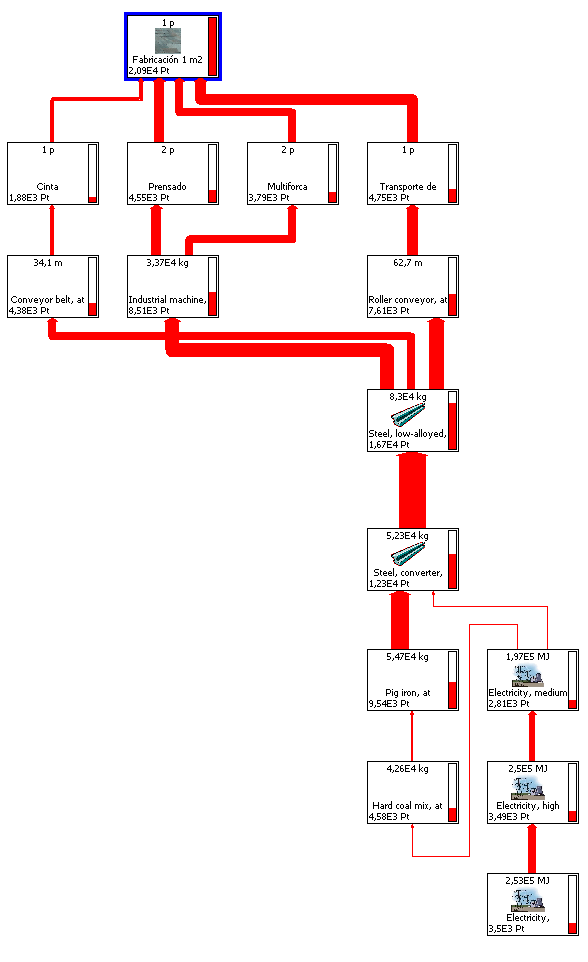
\includegraphics[width=14cm]{img/fabric_red.png}
\caption[Red de la fase de extracción de materias primas, fabricación e instalación.]{Red de la fase de extracción de materias primas, fabricación e instalación. Fuente: elaboración propia.}
\label{fig:fabric_red}
\end{figure}

Cada caja representa un proceso y cada proceso se muestra una única vez. Las flechas representan los flujos entre procesos. Las barras o termómetros indican la carga medioambiental generada en cada proceso y sus procesos aguas arriba. De esta manera se puede distinguir entre los procesos más importantes y los menos, identificando los puntos calientes.

De la red de la fase de extracción de materias primas, fabricación e instalación se puede obtener que la extracción de materias primas para la capa bituminosa y el árido grueso de la capa base de la instalación son los procesos con mayor carga medioambiental de esta fase. También destaca el proceso de fabricación del cemento Portland para la creación del hormigón del adoquín.

La caracterización del análisis de impacto muestra todas las categorías de impacto. Cada una de ellas tiene una unidad de medida diferente, por lo que se representan gráficamente de forma porcentual. Para tener una visión más clara de los impactos relevantes de la fase, es mejor recurrir a la normalización donde las diferentes puntuaciones de los impactos caracterizados se relativizan a una referencia común.

La figura \ref{fig:fabric_normalizacion} y la tabla \ref{categoriasimpactofabricacion} muestran las categorías de impacto relevantes de esta fase.

\begin{figure}[!htb]
\centering
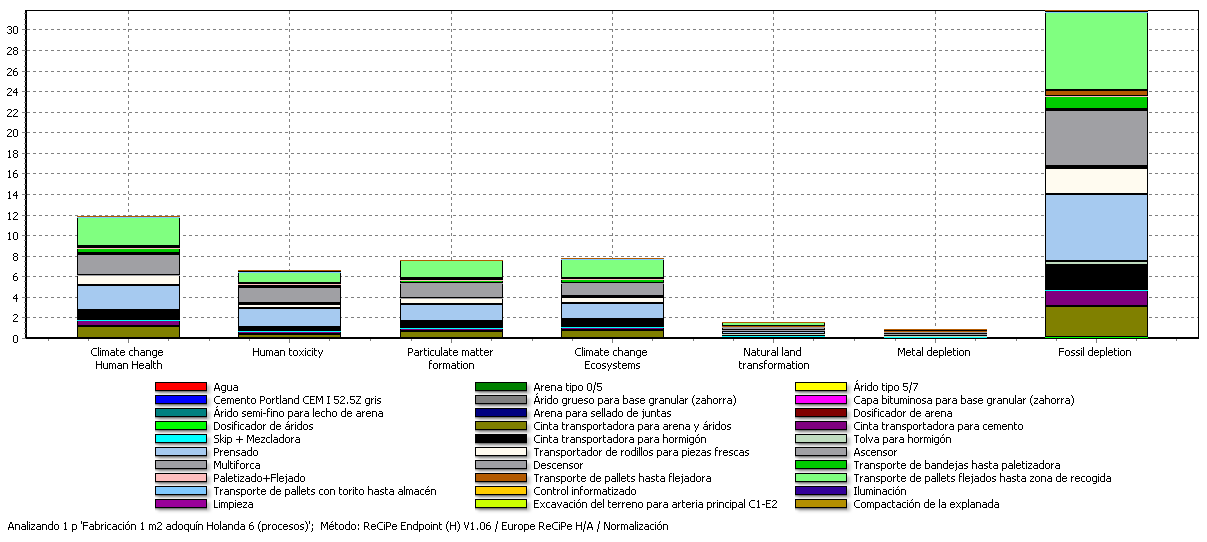
\includegraphics[width=15cm]{img/fabric_normalizacion.png}
\caption[Cuantificación de los impactos normalizados de la fase de extracción de materias primas, fabricación e instalación.]{Cuantificación de los impactos normalizados de la fase de extracción de materias primas, fabricación e instalación. Fuente: elaboración propia.}
\label{fig:fabric_normalizacion}
\end{figure}

La categoría con mayor impacto es la de ``Agotamiento de recursos fósiles'', donde destacan la extracción de materias primas para la capa bituminosa y el árido grueso de la capa base de la instalación y el proceso de fabricación del cemento Portland. Para el resto de categorías de impacto se produce una situación similar. En la categoría de ``Ocupación de tierras agrícolas'' presenta cierta relevancia el proceso de paletizado y flejado de los pallets debido a la tala de árboles para la fabricación de madera y papel.

\begin{table}[!htb]
\centering
\begin{tabular}{p{4cm}rrrrrrr}
\toprule
\multicolumn{8}{c}{Categorías de impacto normalizadas}\\
\midrule
Proceso & CC[HH] & HT & PMF & CC[Ec] & ALO & NLT & FD\\
 &  (\%) & (\%) & (\%) & (\%) & (\%) & (\%) & (\%)\\
\midrule
Capa bituminosa para base granular & 23.2 & 17.0 & 16.5 & 23.2 & 3.09 & 30.5 & 55.2\\
Árido grueso para base granular & 26.8 & 28.9 & 46.9 & 26.8 & 65.2 & 35.4 & 21.3\\
Cemento Portland CEM I gris & 27.4 & 9.62 & 8.13 & 27.4 & 0.21 & 1.48 & 6.67\\
Paletizado y flejado & 3.2 & 9.42 & 3.78 & 3.2 & 31.2 & 14.4 & 2.36\\
Sellado y vibrado del pavimento & 4.56 & 0.79 & 8.1 & 4.56 & 0.01 & 2.62 & 3.69\\
\bottomrule
\end{tabular}
\caption[Categorías de impacto normalizadas de la fase de extracción de materias primas, fabricación e instalación.]{Categorías de impacto normalizadas de la fase de extracción de materias primas, fabricación e instalación. CC[HH]: cambio climático—salud humana, HT: toxicidad humana, PMF: formación de partículas, CC[Ec]: cambio climático—ecosistema, ALO: ocupación de tierras agrícolas, NLT: transformación natural de la tierra, FD: agotamiento de recursos fósiles. Fuente: elaboración propia.}
\label{categoriasimpactofabricacion}
\end{table}

La puntuación única permite observar los resultados desde una perspectiva diferente. Esta opción agrupa las categorías de impacto aplicando una serie de puntos a cada una, representando finalmente todas las categorías de impacto usando una misma unidad, el punto (\textit{Point}, Pt). La carga ambiental será mayor cuanto más Pt tenga.

\begin{figure}[!htb]
\centering
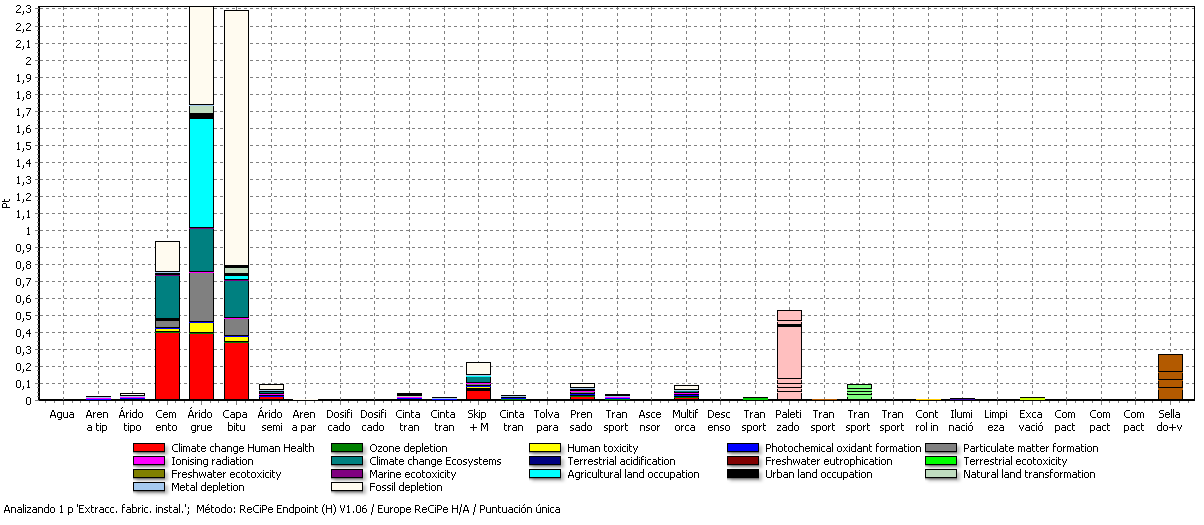
\includegraphics[width=15cm]{img/fabric_puntuacionunica.png}
\caption[Cuantificación de los impactos a nivel de puntuación única de la fase de extracción de materias primas, fabricación e instalación.]{Cuantificación de los impactos a nivel de puntuación única de la fase de extracción de materias primas, fabricación e instalación. Fuente: elaboración propia.}
\label{fig:fabric_puntuacionunica}
\end{figure}

La figura \ref{fig:fabric_puntuacionunica} muestra las categorías de impacto a nivel de puntuación única. Los resultados son similares a los de la normalización, donde la extracción de materias primas para la capa bituminosa y el árido grueso de la capa base de la instalación y el proceso de fabricación del cemento Portland tienen la mayor puntuación (ver tabla \ref{categoriasimpactofabricacionpuntunica}).

\begin{table}[!htb]
\centering
\begin{tabular}{p{4cm}rrrrrrr}
\toprule
\multicolumn{8}{c}{Categorías de impacto puntuación final}\\
\midrule
Proceso & CC[HH] & HT & PMF & CC[Ec] & ALO & NLT & FD\\
 &  (\%) & (\%) & (\%) & (\%) & (\%) & (\%) & (\%)\\
\midrule
Capa bituminosa para base granular & 23.2 & 17.0 & 16.5 & 23.2 & 3.09 & 30.5 & 55.2\\
Árido grueso para base granular & 26.8 & 28.9 & 46.9 & 26.8 & 65.2 & 35.4 & 21.3\\
Cemento Portland CEM I gris & 27.4 & 9.62 & 8.13 & 27.4 & 0.21 & 1.48 & 6.67\\
Paletizado y flejado & 3.2 & 9.42 & 3.78 & 3.2 & 31.2 & 14.4 & 2.36\\
Sellado y vibrado del pavimento & 4.56 & 0.79 & 8.1 & 4.56 & 0.01 & 2.62 & 3.69\\
\bottomrule
\end{tabular}
\caption[Categorías de impacto a nivel de puntuación única de la fase de extracción de materias primas, fabricación e instalación.]{Categorías de impacto a nivel de puntuación única de la fase de extracción de materias primas, fabricación e instalación. CC[HH]: cambio climático—salud humana, HT: toxicidad humana, PMF: formación de partículas, CC[Ec]: cambio climático—ecosistema, ALO: ocupación de tierras agrícolas, NLT: transformación natural de la tierra, FD: agotamiento de recursos fósiles. Fuente: elaboración propia.}
\label{categoriasimpactofabricacionpuntunica}
\end{table}

Atendiendo a las categorías de daños (punto final) de la tabla \ref{categoriasdanosfabricacion}, los resultados indican que el mayor daño se produce en el aspecto de recursos.

\begin{table}[!htb]
\centering
\begin{tabular}{p{6cm}rrrr}
\toprule
\multicolumn{5}{c}{Categorías de daño puntuación única}\\
\midrule
Proceso & Salud hum. & Ecosistema & Recursos & Total\\
 & (Pt) & (Pt) &  (Pt) & (Pt)\\
\midrule
Capa bituminosa para base granular & 0.482 & 0.302 & 1.510 & 2.290\\
Árido grueso para base granular & 0.753 & 0.979 & 0.582 & 2.310\\
Cemento Portland CEM I gris & 0.473 & 0.277 & 0.182 & 0.932\\
Paletizado y flejado & 0.093 & 0.370 & 0.065 & 0.527\\
Sellado y vibrado del pavimento & 0.119 & 0.048 & 0.101 & 0.268\\
\midrule
Total (Pt) & 2.32 & 2.15 & 2.74 & \textbf{7.21}\\
\bottomrule
\end{tabular}
\caption[Puntuación única por categorías de daños de la fase de extracción de materias primas, fabricación e instalación.]{Puntuación única por categorías de daños de la fase de extracción de materias primas, fabricación e instalación. Fuente: elaboración propia.}
\label{categoriasdanosfabricacion}
\end{table}

\section{Evaluación del Impacto Ambiental de la fase de uso y mantenimiento}

La red de la fase de uso y mantenimiento de la figura \ref{fig:uso_red} muestra todos los procesos interrelacionados para dar una perspectiva general de la fase.

\begin{figure}[!htb]
\centering
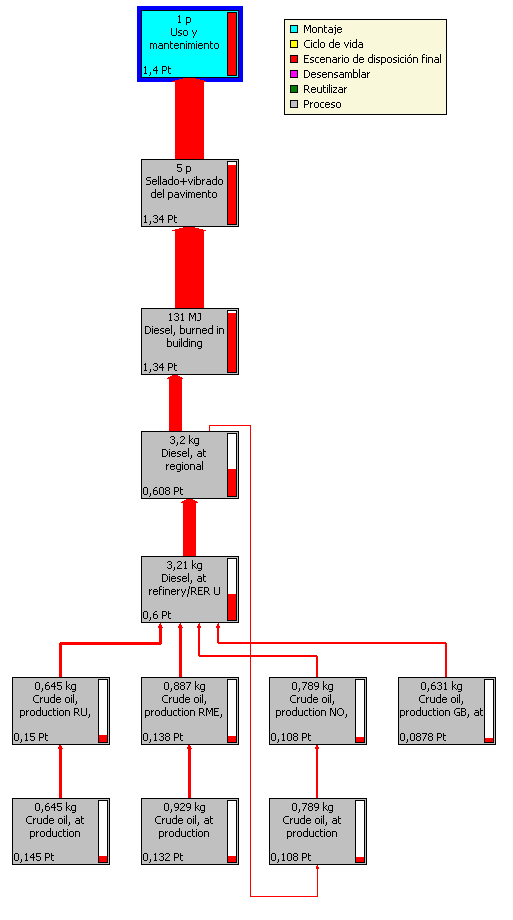
\includegraphics[width=5cm]{img/uso_red.png}
\caption[Red de la fase de uso y mantenimiento.]{Red de la fase de uso y mantenimiento. Fuente: elaboración propia.}
\label{fig:uso_red}
\end{figure}

Cada caja representa un proceso y cada proceso se muestra una única vez. Las flechas representan los flujos entre procesos. Las barras o termómetros indican la carga medioambiental generada en cada proceso y sus procesos aguas arriba. De esta manera se puede distinguir entre los procesos más importantes y los menos, identificando los puntos calientes.

Del análisis de la red de la fase de uso y mantenimiento se obtiene que el proceso con mayor carga ambiental es el sellado y vibrado del pavimento.

La caracterización del análisis de impacto muestra todas las categorías de impacto. Cada una de ellas tiene una unidad de medida diferente, por lo que se representan gráficamente de forma porcentual. Para tener una visión más clara de los impactos relevantes de la fase, es mejor recurrir a la normalización donde las diferentes puntuaciones de los impactos caracterizados se relativizan a una referencia común.

La figura \ref{fig:uso_normalizacion} y la tabla \ref{categoriasimpactouso} muestran las categorías de impacto relevantes de esta fase.

\begin{figure}[!htb]
\centering
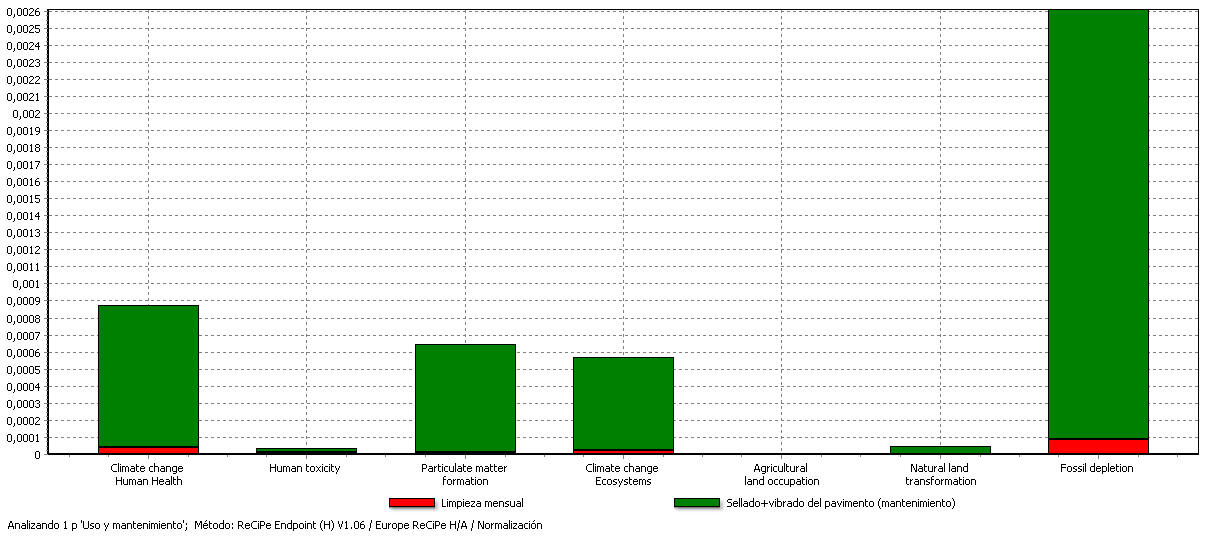
\includegraphics[width=15cm]{img/uso_normalizacion.png}
\caption[Cuantificación de los impactos normalizados de la fase de uso y mantenimiento.]{Cuantificación de los impactos normalizados de la fase de uso y mantenimiento. Fuente: elaboración propia.}
\label{fig:uso_normalizacion}
\end{figure}

Al igual que en la fase de extracción de materias primas, fabricación e instalación, la categoría con mayor impacto es la de ``Agotamiento de recursos fósiles'', donde el sellado y vibrado del pavimento es el proceso dominante. El resto de categorías de impacto muestran la misma situación.

\begin{table}[!htb]
\centering
\begin{tabular}{p{4cm}rrrrrrr}
\toprule
\multicolumn{8}{c}{Categorías de impacto normalizadas}\\
\midrule
Proceso & CC[HH] & HT & PMF & CC[Ec] & ALO & NLT & FD\\
 &  (\%) & (\%) & (\%) & (\%) & (\%) & (\%) & (\%)\\
\midrule
Limpieza mensual & 4.54 & 38.6 & 1.75 & 4.54 & 71.4 & 3.57 & 3.48\\
Sellado y vibrado & 95.5 & 61.4 & 98.2 & 95.5 & 28.6 & 96.4 & 96.5\\
\bottomrule
\end{tabular}
\caption[Categorías de impacto normalizadas de la fase de uso y mantenimiento.]{Categorías de impacto normalizadas de la fase de uso y mantenimiento. CC[HH]: cambio climático—salud humana, HT: toxicidad humana, PMF: formación de partículas, CC[Ec]: cambio climático—ecosistema, ALO: ocupación de tierras agrícolas, NLT: transformación natural de la tierra, FD: agotamiento de recursos fósiles. Fuente: elaboración propia.}
\label{categoriasimpactouso}
\end{table}

La puntuación única permite observar los resultados desde una perspectiva diferente. Esta opción agrupa las categorías de impacto aplicando una serie de puntos a cada una, representando finalmente todas las categorías de impacto usando una misma unidad, el punto (\textit{Point}, Pt). La carga ambiental será mayor cuanto más Pt tenga.

\begin{figure}[!htb]
\centering
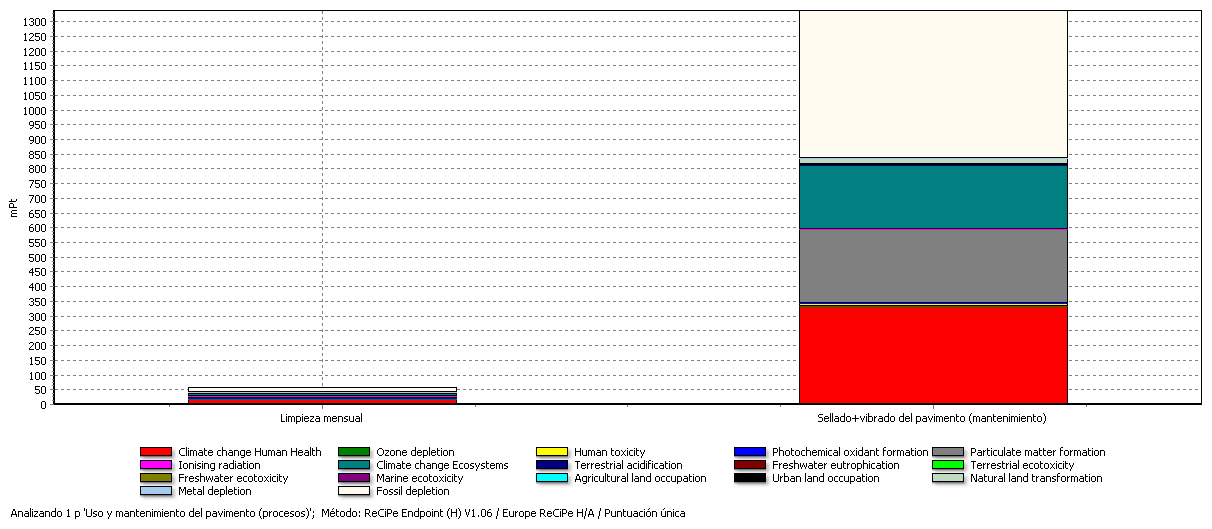
\includegraphics[width=15cm]{img/uso_puntuacionunica.png}
\caption[Cuantificación de los impactos a nivel de puntuación única de uso y mantenimiento.]{Cuantificación de los impactos a nivel de puntuación única de uso y mantenimiento. Fuente: elaboración propia.}
\label{fig:uso_puntuacionunica}
\end{figure}

La figura \ref{fig:uso_puntuacionunica} muestra las categorías de impacto a nivel de puntuación única. Los resultados son similares a los de la normalización. El proceso de sellado y vibrado del pavimento afecta principalmente a las categorías de agotamiento de recursos fósiles y al cambio climático desde el punto de vista de la salud humana. En menor medida afecta al cambio climática visto desde el ecosistema y a la formación de partículas (ver tabla \ref{categoriasimpactousopuntunica}).

\begin{table}[!htb]
\centering
\begin{tabular}{p{4cm}rrrrrrr}
\toprule
\multicolumn{8}{c}{Categorías de impacto puntuación única}\\
\midrule
Proceso & CC[HH] & HT & PMF & CC[Ec] & ALO & NLT & FD\\
 &  (\%) & (\%) & (\%) & (\%) & (\%) & (\%) & (\%)\\
\midrule
Limpieza & 4.54 & 38.6 & 1.75 & 4.54 & 54.1 & 3.57 & 3.48\\
Sellado y vibrado & 95.5 & 61.4 & 98.2 & 95.5 & 28.6 & 96.4 & 96.5\\
\bottomrule
\end{tabular}
\caption[Categorías de impacto a nivel de puntuación única de la fase de uso y mantenimiento.]{Categorías de impacto a nivel de puntuación única de la fase de uso y mantenimiento. CC[HH]: cambio climático—salud humana, HT: toxicidad humana, PMF: formación de partículas, CC[Ec]: cambio climático—ecosistema, ALO: ocupación de tierras agrícolas, NLT: transformación natural de la tierra, FD: agotamiento de recursos fósiles. Fuente: elaboración propia.}
\label{categoriasimpactousopuntunica}
\end{table}

Atendiendo a las categorías de daños (punto final) de la tabla \ref{categoriasdanosuso}, los resultados indican que el mayor daño se produce en la salud humana.

\begin{table}[!htb]
\centering
\begin{tabular}{p{6cm}rrrr}
\toprule
\multicolumn{5}{c}{Categorías de daño puntuación única}\\
\midrule
Proceso & Salud hum. & Ecosistema & Recursos & Total\\
 & (Pt) & (Pt) &  (Pt) & (Pt)\\
\midrule
Limpieza & 0.0262 & 0.0134 & 0.0182 & 0.0577\\
Sellado y vibrado & 0.5940 & 0.2400 & 0.5040 & 1.3400\\
\midrule
Total (Pt) & 0.621 & 0.253 & 0.522 & \textbf{1.4}\\
\bottomrule
\end{tabular}
\caption[Puntuación única por categorías de daños de la fase de uso y mantenimiento.]{Puntuación única por categorías de daños de la fase de uso y mantenimiento. Fuente: elaboración propia.}
\label{categoriasdanosuso}
\end{table}

\section{Evaluación del Impacto Ambiental de la fase de fin de vida}

En la red de la fase de fin de vida de la figura \ref{fig:fdv_red} se muestran todos los procesos interrelacionados para dar una perspectiva general de la fase.

\begin{figure}[!htb]
\centering
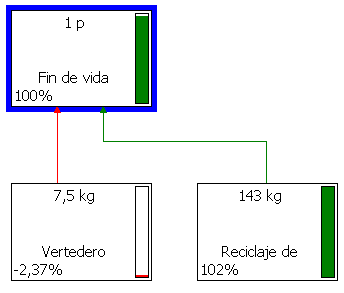
\includegraphics[width=5cm]{img/fdv_red.png}
\caption[Red de la fase de fin de vida.]{Red de la fase de fin de vida. Fuente: elaboración propia.}
\label{fig:fdv_red}
\end{figure}

Cada caja representa un proceso y cada proceso se muestra una única vez. Las flechas representan los flujos entre procesos. Las barras o termómetros indican la carga medioambiental generada en cada proceso y sus procesos aguas arriba. De esta manera se puede distinguir entre los procesos más importantes y los menos, identificando los puntos calientes.

En la red de la fase de fin de vida los procesos se muestran termómetros verdes en lugar de rojos, ya que se tiene en cuenta el beneficio ambiental del proceso de reciclaje del adoquín en árido, por lo que el vertedero tiene un beneficio negativo, es decir un impacto ambiental.

La caracterización del análisis de impacto muestra todas las categorías de impacto. Cada una de ellas tiene una unidad de medida diferente, por lo que se representan gráficamente de forma porcentual. Para tener una visión más clara de los impactos relevantes de la fase, es mejor recurrir a la normalización donde las diferentes puntuaciones de los impactos caracterizados se relativizan a una referencia común.

La figura \ref{fig:fdv_normalizacion} y la tabla \ref{categoriasimpactofdv} muestran las categorías de impacto relevantes de esta fase.

\begin{figure}[!htb]
\centering
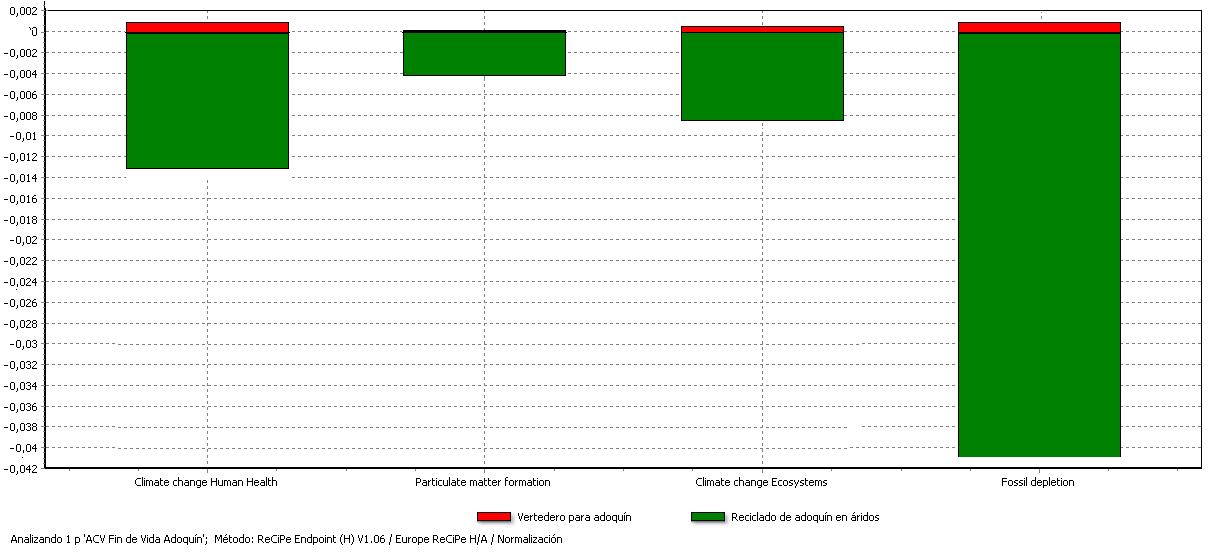
\includegraphics[width=15cm]{img/fdv_normalizacion.png}
\caption[Cuantificación de los impactos normalizados de la fase de fin de vida.]{Cuantificación de los impactos normalizados de la fase de fin de vida. Fuente: elaboración propia.}
\label{fig:fdv_normalizacion}
\end{figure}

A diferencia de las dos fases anteriores, se produce un beneficio, principalmente en la categoría de ``Agotamiento de recursos fósiles'', donde el reciclaje de adoquín en árido supone un producto evitado, el árido, cuya carga ambiental es negativa (beneficio ambiental).

\begin{table}[!htb]
\centering
\begin{tabular}{p{4cm}rrrrrrr}
\toprule
\multicolumn{8}{c}{Categorías de impacto normalizadas}\\
\midrule
Proceso & CC[HH] & HT & PMF & CC[Ec] & ALO & NLT & FD\\
 &  (\%) & (\%) & (\%) & (\%) & (\%) & (\%) & (\%)\\
\midrule
Vertedero & 1.65 & 1.01 & 3.51 & 1.65 & 6.88 & -10.6 & 4.52\\
Reciclaje de adoquín en árido & -102 & -101 & -104 & -102 & -07 & -89.4 & -105\\
\bottomrule
\end{tabular}
\caption[Categorías de impacto normalizadas de la fase de fin de vida.]{Categorías de impacto normalizadas de la fase de fin de vida. CC[HH]: cambio climático—salud humana, HT: toxicidad humana, PMF: formación de partículas, CC[Ec]: cambio climático—ecosistema, ALO: ocupación de tierras agrícolas, NLT: transformación natural de la tierra, FD: agotamiento de recursos fósiles. Fuente: elaboración propia.}
\label{categoriasimpactofdv}
\end{table}

La puntuación única permite observar los resultados desde una perspectiva diferente. Esta opción agrupa las categorías de impacto aplicando una serie de puntos a cada una, representando finalmente todas las categorías de impacto usando una misma unidad, el punto (\textit{Point}, Pt). La carga ambiental será mayor cuanto más Pt tenga.

\begin{figure}[!htb]
\centering
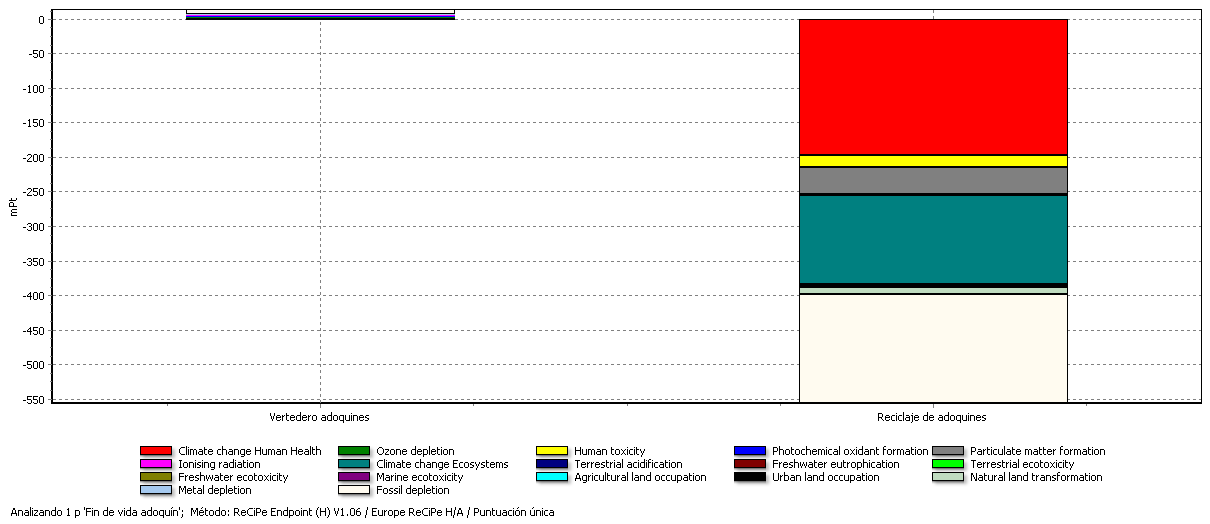
\includegraphics[width=15cm]{img/fdv_puntuacionunica.png}
\caption[Cuantificación de los impactos a nivel de puntuación única de fin de vida.]{Cuantificación de los impactos a nivel de puntuación única de fin de vida. Fuente: elaboración propia.}
\label{fig:fdv_puntuacionunica}
\end{figure}

La figura \ref{fig:fdv_puntuacionunica} muestra las categorías de impacto a nivel de puntuación única. Los resultados son coherentes con los de la normalización. El proceso de reciclaje de adoquín en áridos aporta un beneficio principalmente a las categorías de agotamiento de recursos fósiles y al cambio climático desde el punto de vista de la salud humana. También beneficia, en menor proporción, al cambio climática visto desde el ecosistema y a la formación de partículas (ver tabla \ref{categoriasimpactofdvpuntunica}).

\begin{table}[!htb]
\centering
\begin{tabular}{p{4cm}rrrrrrr}
\toprule
\multicolumn{8}{c}{Categorías de impacto puntuación única}\\
\midrule
Proceso & CC[HH] & HT & PMF & CC[Ec] & ALO & NLT & FD\\
 &  (\%) & (\%) & (\%) & (\%) & (\%) & (\%) & (\%)\\
\midrule
Vertedero & 1.65 & 1.01 & 3.51 & 1.65 & 6.88 & -10.6 & 4.52\\
Reciclaje de adoquín en árido & -102 & -101 & -104 & -102 & -07 & -89.4 & -105\\
\bottomrule
\end{tabular}
\caption[Categorías de impacto a nivel de puntuación única de la fase de fin de vida.]{Categorías de impacto a nivel de puntuación única de la fase de fin de vida. CC[HH]: cambio climático—salud humana, HT: toxicidad humana, PMF: formación de partículas, CC[Ec]: cambio climático—ecosistema, ALO: ocupación de tierras agrícolas, NLT: transformación natural de la tierra, FD: agotamiento de recursos fósiles. Fuente: elaboración propia.}
\label{categoriasimpactofdvpuntunica}
\end{table}

Atendiendo a las categorías de daños (punto final) de la tabla \ref{categoriasdanosfdv}, los resultados indican que el mayor beneficio se produce en el aspecto de recursos.

\begin{table}[!htb]
\centering
\begin{tabular}{p{6cm}rrrr}
\toprule
\multicolumn{5}{c}{Categorías de daño puntuación única}\\
\midrule
Proceso & Salud hum. & Ecosistema & Recursos & Total\\
 & (Pt) & (Pt) & (Pt) & (Pt)\\
\midrule
Vertedero & 0.00473 & 0.00136 & 0.00681 & 0.0129\\
Reciclaje de adoquín en árido & -0.255 & -0.143 & -0.158 & -0.556\\
\midrule
Total (Pt) & -0.251 & -0.142 & -0.151 & \textbf{-0.543}\\
\bottomrule
\end{tabular}
\caption[Categorías de daños de la fase de fin de vida.]{Categorías de daños de la fase de fin de vida. Fuente: elaboración propia.}
\label{categoriasdanosfdv}
\end{table}

\section{Evaluación del Impacto Ambiental del ciclo de vida completo}

Una vez estudiadas las tres fases del ciclo de vida se procederá a realizar un análisis completo del producto a lo largo de las tres fases anteriores de su ciclo de vida.

A priori, observando los resultados ya obtenidos en las tablas de categorías de impacto \ref{categoriasimpactofabricacion}, \ref{categoriasimpactouso} y \ref{categoriasimpactofdv}, se puede asegurar que las etapas de uso y mantenimiento y fin de vida tienen menores consecuencias comparadas con la de extracción de materias primas, fabricación e instalación.

La red del ciclo de vida completo de la figura \ref{fig:completo_red} demuestra que la únicamente la fase de extracción de materias primas, fabricación e instalación representa un impacto del 89.4\%, mientras que la de uso y mantenimiento aporta un 17.3\% y la de fin de vida un beneficio del 6.74\%.

\begin{figure}[!htb]
\centering
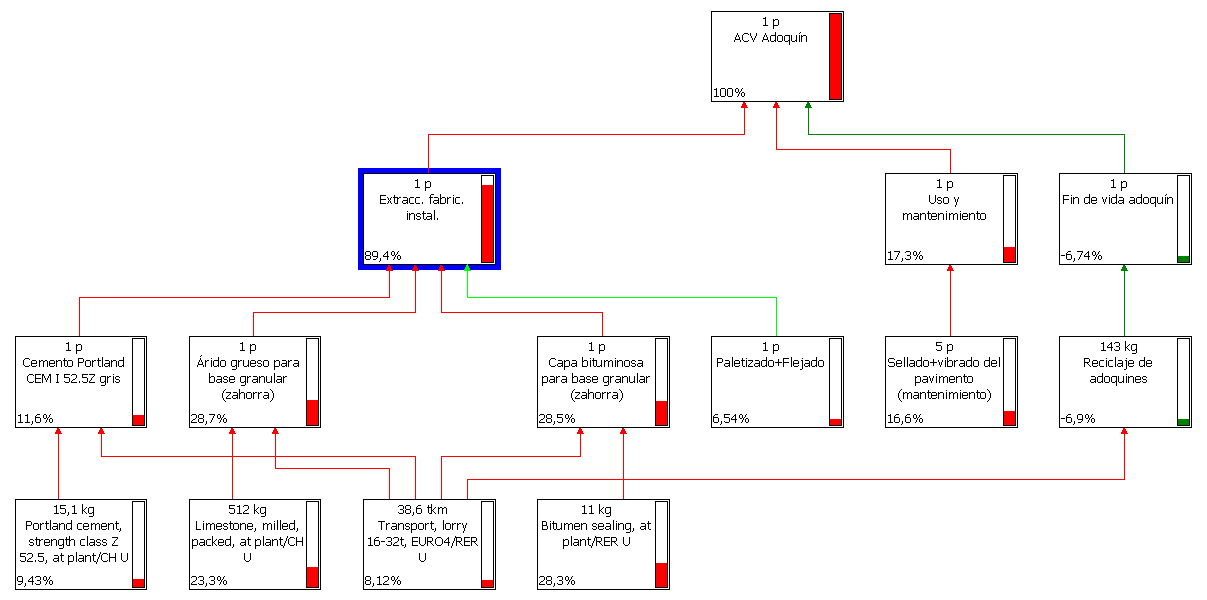
\includegraphics[width=14cm]{img/completo_red.png}
\caption[Red del ciclo de vida completo.]{Red del ciclo de vida completo. Fuente: elaboración propia.}
\label{fig:completo_red}
\end{figure}

Cada caja representa un proceso y cada proceso se muestra una única vez. Las flechas representan los flujos entre procesos. Las barras o termómetros indican la carga medioambiental generada en cada proceso y sus procesos aguas arriba. Si el termómetro es de color verde indica que es un beneficio ambiental. De esta manera se puede distinguir entre los procesos más importantes y los menos, identificando los puntos calientes.

La caracterización del análisis de impacto de la figura \ref{fig:completo_caracterizacion} y la tabla \ref{categoriasimpactocompletocaracterizados} muestra todas las categorías de impacto. Cada una de ellas tiene una unidad de medida diferente, por lo que se representan de forma porcentual.

\begin{figure}[!htb]
\centering
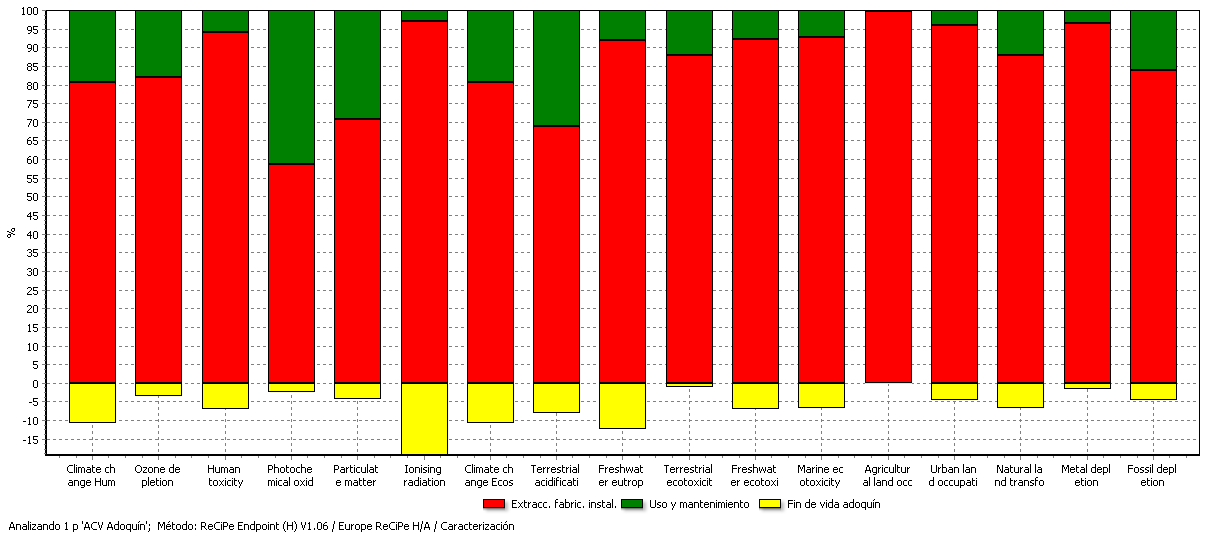
\includegraphics[width=15cm]{img/completo_caracterizacion.png}
\caption[Cuantificación de los impactos caracterizados del ciclo de vida completo.]{Cuantificación de los impactos caracterizados del ciclo de vida completo. Fuente: elaboración propia.}
\label{fig:completo_caracterizacion}
\end{figure}

\begin{table}[!htb]
\centering
\begin{tabular}{p{2cm}rrrrrrrrr}
\toprule
\multicolumn{10}{c}{Categorías de impacto caracterizadas}\\
\midrule
Proceso & CC[HH] & OD & HT & POF & PMF & IR & CC[Ec] & TA & FE\\
 &  (\%) & (\%) & (\%) & (\%) & (\%) & (\%) & (\%) & (\%) & (\%)\\
\midrule
Ex-fab-inst. & 90.4 & 85.1 & 101 & 60.1 & 74 & 120 & 90.4 & 75.1& 105\\
Uso-mant. & 21.6 & 18.6 & 6.46 & 42.3 & 30.5 & 3.71 & 21.6 & 33.9 & 9.18\\
Fin-vida & -12 & -3.72 & -7.45 & -2.47 & -4.56 & -24 & -12 & -8.93 & -14\\
\midrule
\midrule
Proceso & TE & FE & ME & ALO & ULO & NLT & MD & FD\\
 &  (\%) & (\%) & (\%) & (\%) & (\%) & (\%) & (\%) & (\%)\\
\midrule
Ex-fab-inst. & 88.8 & 99.4 & 99.4 & 100 & 100 & 94.4 & 98.1 & 88\\
Uso-mant. & 12.2 & 8.25 & 7.74 & 0.14 & 4.32 & 12.8 & 3.66 & 16.8\\
Fin-vida & -1.01 & -7.65 & -7.18 & -0.09 & -4.78 & -7.21 & -1.74 & -4.85\\
\bottomrule
\end{tabular}
\caption[Categorías de impacto caracterizadas del ciclo de vida completo.]{Categorías de impacto caracterizadas del ciclo de vida completo. CC[HH]: cambio climático—salud humana, OD: Agotamiento de ozono, HT: toxicidad humana, POF: formación de oxidantes fotoquímicos, PMF: formación de partículas, IR: radiaciones ionizantes, CC[Ec]: cambio climático—ecosistema, TA: acidificación terrestre, FE: eutrofización del agua dulce, TE: ecotoxicidad terrestre, FE: ecotoxicidad del agua dulce, ME: ecotoxicidad marina, ALO: ocupación de tierras agrícolas, ULO: ocupación de suelo urbano, NLT: transformación natural de la tierra, MD: agotamiento de recursos minerales, FD: agotamiento de recursos fósiles. Fuente: elaboración propia.}
\label{categoriasimpactocompletocaracterizados}
\end{table}

Para tener una visión más clara de los impactos relevantes de la fase, es mejor recurrir a la normalización donde las diferentes puntuaciones de los impactos caracterizados se relativizan a una referencia común.

La figura \ref{fig:completo_normalizacion} y la tabla \ref{categoriasimpactocompleto} muestran las categorías de impacto relevantes de esta fase.

\begin{figure}[!htb]
\centering
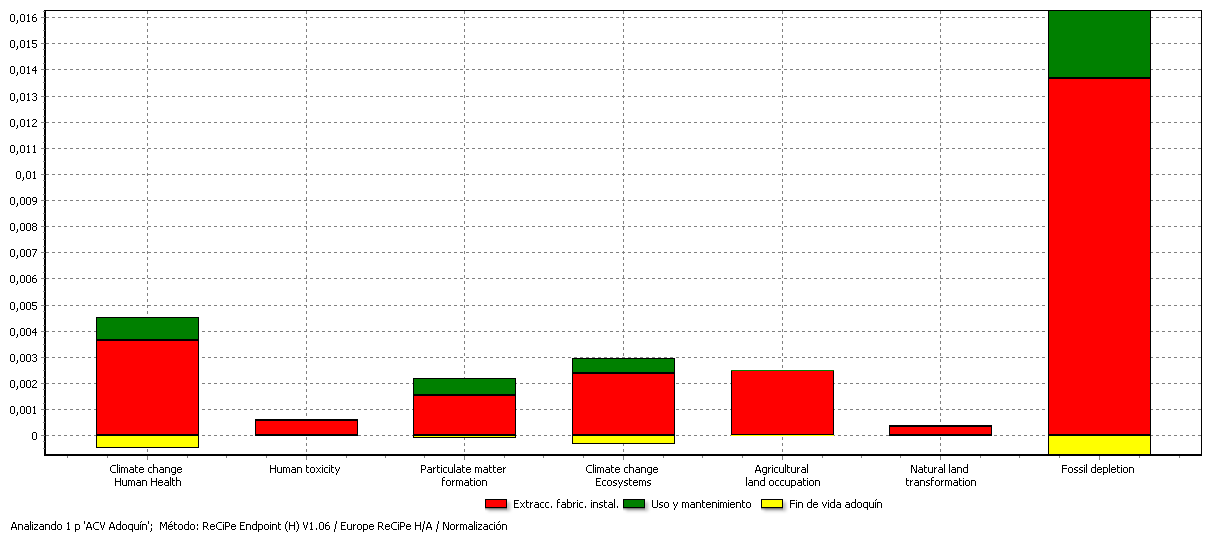
\includegraphics[width=15cm]{img/completo_normalizacion.png}
\caption[Cuantificación de los impactos normalizados del ciclo de vida completo.]{Cuantificación de los impactos normalizados del ciclo de vida completo. Fuente: elaboración propia.}
\label{fig:completo_normalizacion}
\end{figure}

La categoría con mayor impacto es la de ``Agotamiento de recursos fósiles'', donde la fase que predomina es la de extracción de materias primas, fabricación e instalación en todas las categorías de impacto (ver figura \ref{fig:completo_normalizacion}).

\begin{table}[!htb]
\centering
\begin{tabular}{p{4cm}rrrrrrr}
\toprule
\multicolumn{8}{c}{Categorías de impacto normalizadas}\\
\midrule
Proceso & CC[HH] & HT & PMF & CC[Ec] & ALO & NLT & FD\\
 &  (\%) & (\%) & (\%) & (\%) & (\%) & (\%) & (\%)\\
\midrule
Extracc., fabric. e instal. & 90.4 & 101 & 74 & 90.4 & 100 & 94.4 & 88\\
Uso y mantenim. & 21.6 & 6.46 & 30.5 & 21.6 & 0.14 & 12.8 & 16.8\\
Fin de vida & -12 & -7.45 & -4.56 & -12 & -0.09 & -7.21 & -4.85\\
\bottomrule
\end{tabular}
\caption[Categorías de impacto normalizadas del ciclo de vida completo.]{Categorías de impacto normalizadas del ciclo de vida completo. CC[HH]: cambio climático—salud humana, HT: toxicidad humana, PMF: formación de partículas, CC[Ec]: cambio climático—ecosistema, ALO: ocupación de tierras agrícolas, NLT: transformación natural de la tierra, FD: agotamiento de recursos fósiles. Fuente: elaboración propia.}
\label{categoriasimpactocompleto}
\end{table}

Los datos ponderados de la tabla \ref{categoriasimpactocompletoponderados} indican resultados similares a la normalización.

\begin{table}[!htb]
\centering
\begin{tabular}{p{4cm}rrrrrrr}
\toprule
\multicolumn{8}{c}{Categorías de impacto ponderadas}\\
\midrule
Proceso & CC[HH] & HT & PMF & CC[Ec] & ALO & NLT & FD\\
 &  (\%) & (\%) & (\%) & (\%) & (\%) & (\%) & (\%)\\
\midrule
Extracc., fabric. e instal. & 90.4 & 101 & 74 & 90.4 & 100 & 94.4 & 88\\
Uso y mantenim. & 21.6 & 6.46 & 30.5 & 21.6 & 0.14 & 12.8 & 16.8\\
Fin de vida & -12 & -7.45 & -4.56 & -12 & -0.09 & -7.21 & -4.85\\
\bottomrule
\end{tabular}
\caption[Categorías de impacto ponderadas del ciclo de vida completo.]{Categorías de impacto ponderadas del ciclo de vida completo. CC[HH]: cambio climático—salud humana, HT: toxicidad humana, PMF: formación de partículas, CC[Ec]: cambio climático—ecosistema, ALO: ocupación de tierras agrícolas, NLT: transformación natural de la tierra, FD: agotamiento de recursos fósiles. Fuente: elaboración propia.}
\label{categoriasimpactocompletoponderados}
\end{table}

La puntuación única permite observar los resultados desde una perspectiva diferente. Esta opción agrupa las categorías de impacto aplicando una serie de puntos a cada una, representando finalmente todas las categorías de impacto usando una misma unidad, el punto (\textit{Point}, Pt). La carga ambiental será mayor cuanto más Pt tenga.

\begin{figure}[!htb]
\centering
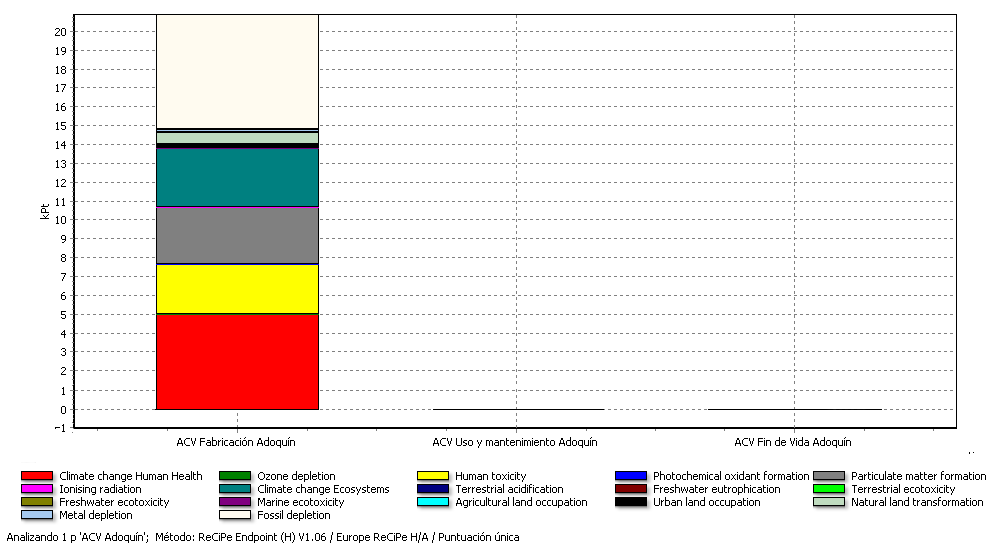
\includegraphics[width=15cm]{img/completo_puntuacionunica.png}
\caption[Cuantificación de los impactos a nivel de puntuación única del ciclo de vida completo.]{Cuantificación de los impactos a nivel de puntuación única del ciclo de vida completo. Fuente: elaboración propia.}
\label{fig:completo_puntuacionunica}
\end{figure}

La figura \ref{fig:completo_puntuacionunica} muestra las categorías de impacto a nivel de puntuación única. Los resultados son similares a los de la normalización, donde la fase de extracción de materias primas, fabricación e instalación tiene la mayor puntuación (ver tabla \ref{categoriasimpactocompletopuntunica}).

\begin{table}[!htb]
\centering
\begin{tabular}{p{4cm}rrrrrrr}
\toprule
\multicolumn{8}{c}{Categorías de impacto puntuación única}\\
\midrule
Proceso & CC[HH] & HT & PMF & CC[Ec] & ALO & NLT & FD\\
 &  (\%) & (\%) & (\%) & (\%) & (\%) & (\%) & (\%)\\
\midrule
Extracc., fabric. e instal. & 90.4 & 101 & 74 & 90.4 & 100 & 94.4 & 88\\
Uso y mantenim. & 21.6 & 6.46 & 30.5 & 21.6 & 0.14 & 12.8 & 16.8\\
Fin de vida & -12 & -7.45 & -4.56 & -12 & -0.09 & -7.21 & -4.85\\
\bottomrule
\end{tabular}
\caption[Categorías de impacto a nivel de puntuación única del ciclo de vida completo.]{Categorías de impacto a nivel de puntuación única del ciclo de vida completo. CC[HH]: cambio climático—salud humana, HT: toxicidad humana, PMF: formación de partículas, CC[Ec]: cambio climático—ecosistema, ALO: ocupación de tierras agrícolas, NLT: transformación natural de la tierra, FD: agotamiento de recursos fósiles. Fuente: elaboración propia.}
\label{categoriasimpactocompletopuntunica}
\end{table}

Atendiendo a las categorías de daños (punto final) de la tabla \ref{categoriasdanoscompleto}, los resultados indican que el mayor daño se produce en la salud humana.

\begin{table}[!htb]
\centering
\begin{tabular}{p{6cm}rrrr}
\toprule
\multicolumn{5}{c}{Categorías de daño puntuación única}\\
\midrule
Proceso & Salud hum. & Ecosistema & Recursos & Total\\
 & (Pt) & (Pt) &  (Pt) & (Pt)\\
\midrule
Extracc., fabric. e instal. & 2.32 & 2.15 & 2.74 & 7.21\\
Uso y mantenim. & 0.621 & 0.253 & 0.522 & 1.4\\
Fin de vida & -0.251 & -0.142 & -0.151 & -0.543\\
\midrule
Total (Pt) & 2.69 & 2.26 & 3.11 & \textbf{8.06}\\
\bottomrule
\end{tabular}
\caption[Puntuación única por categorías de daños del ciclo de vida completo.]{Puntuación única por categorías de daños del ciclo de vida completo. Fuente: elaboración propia.}
\label{categoriasdanoscompleto}
\end{table}

De las tablas \ref{categoriasimpactocompleto}, \ref{categoriasimpactocompletoponderados} y \ref{categoriasimpactocompletopuntunica} se puede extraer la conclusión de que la fase que más contribuye al perfil ambiental del adoquín es la de extracción de materias primas, fabricación e instalación. La fase de uso y mantenimiento contribuye lo suficiente como para despreciarla. Por último, la fase de fin de vida aunque contribuye mínimamente, es necesario tenerla en cuenta para cumplir con la Directiva Europea 1999/31/CE relativa al vertido de residuos.

\subsection{Demanda de Energía Acumulada}
A continuación se realizará un análisis de con el método de cálculo de \textbf{Demanda de Energía Acumulada} para conocer la energía que se consume en cada etapa.

La red de la fase de extracción de materias primas, fabricación e instalación de la figura \ref{fig:ced_red} muestra todos los procesos interrelacionados para dar una perspectiva general de la fase.

\begin{figure}[!htbp]
\centering
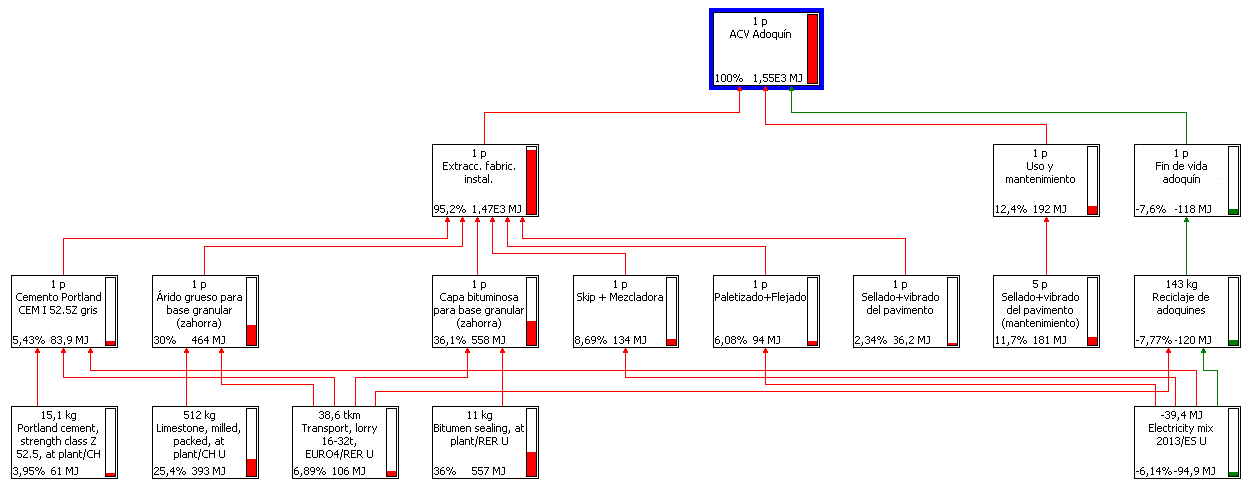
\includegraphics[angle=90,height=18cm]{img/ced_red.png}
\caption[Red del ciclo de vida completo con el método CED.]{Red del ciclo de vida completo con el método CED. Fuente: elaboración propia.}
\label{fig:ced_red}
\end{figure}

Cada caja representa un proceso y cada proceso se muestra una única vez. Las flechas representan los flujos entre procesos. Las barras o termómetros indican la carga medioambiental generada en cada proceso y sus procesos aguas arriba. De esta manera se puede distinguir entre los procesos más importantes y los menos, identificando los puntos calientes.

La figura \ref{fig:ced_puntuacionunica} y la tabla \ref{tiposenergiaced} muestran que existe el mayor consumo de energía se produce en la fase de extracción de materias primas, fabricación e instalación, suponiendo un total del 95.2\% de toda la vida del producto. Por tanto, es esta fase donde hay que mejorar el consumo y en consecuencia su perfil ambiental.

\begin{figure}[!htbp]
\centering
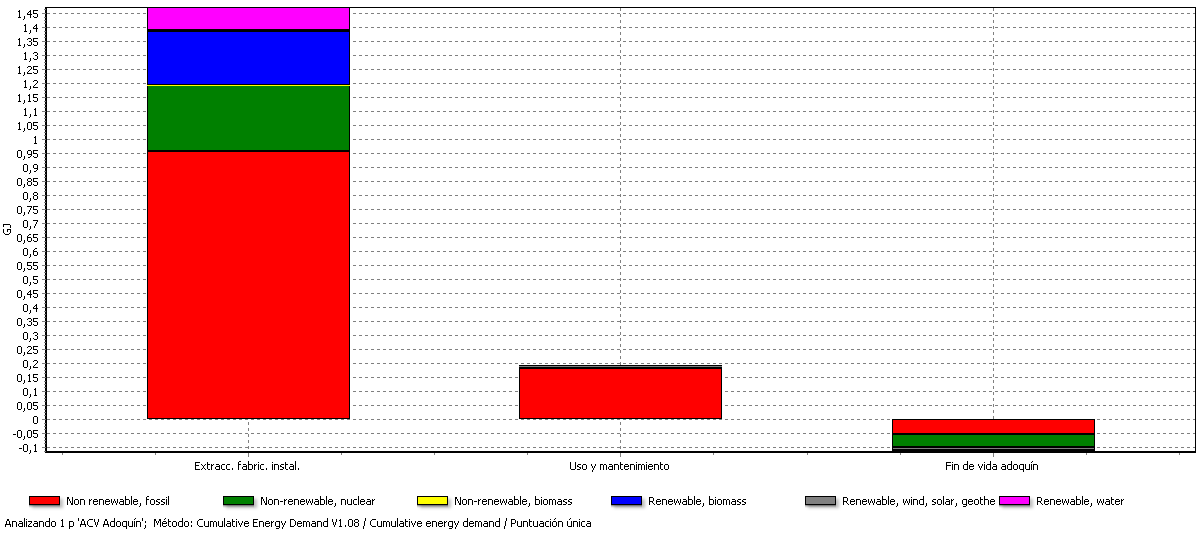
\includegraphics[width=15cm]{img/ced_puntuacionunica.png}
\caption[Cuantificación de los impactos a nivel de puntuación única CED en cada fase.]{Cuantificación de los impactos a nivel de puntuación única CED en cada fase. Fuente: elaboración propia.}
\label{fig:ced_puntuacionunica}
\end{figure}

\begin{table}[!htbp]
\centering
\begin{tabular}{p{2cm}rrrrrrr}
\toprule
\multicolumn{8}{c}{Tipos de energía consumidos}\\
\midrule
 & \multicolumn{3}{c}{No renovables} & \multicolumn{3}{c}{Renovables}\\
\midrule
Etapa & Fósil & Nuclear & Biom. & Biom. & Viento, sol,& Agua\\
 & (\%) & (\%) & (\%) & (\%) & geo (\%) & (\%)\\
\midrule
Ex-fab-inst. & 88 & 120 & 99.7 & 99.8 & 54 & 111\\
Uso-mant. & 16.8 & 3.66 & 0.53 & 0.39 & 2.22 & 1.24\\
Fin-vida & -4.84 & -23.9 & -0.26 & -0.17 & -156 & -12.1\\
\midrule
\midrule
Etapa & Fósil & Nuclear & Biom. & Biom. & Viento, sol,& Agua & Total\\
& (\si{MJ}) & (\si{MJ}) & (\si{MJ}) & (\si{MJ}) & geo (\si{MJ}) & (\si{MJ}) & (\si{MJ})\\
\midrule
Ex-fab-inst. & 958 & 234 & 0.045 & 196 & 3.18 & 80.9 & 1280\\
Uso-mant. & 183 & 7.11 & 0.001 & 0.77 & 0.13 & 0.90 & 192\\
Fin-vida & -52.6 & -46.5 & -0.001 & -0.325 & -9.2 & -8.84 & -118\\
\midrule
Total (\si{MJ}) & 1040 & 176 & 0.024 & 70.2 & -6.11 & 65-2 & \textbf{1350}\\
\bottomrule
\end{tabular}
\caption[Tipos de energía consumidos en cada fase.]{Tipos de energía consumidos en cada fase. Fuente: elaboración propia.}
\label{tiposenergiaced}
\end{table}

La fase de fin de vida aporta un pequeño beneficio del 7.6\% de la energía total consumida en la vida del producto.

\subsection{Cálculo del Potencial de Calentamiento Global}
Finalmente, se utiliza el método IPCC para el cálculo potencial del calentamiento global a lo largo del ciclo de vida. Se aplicará un horizonte temporal a 100 años (GWP 100a) para conocer los kilogramos de \ce{CO2} equivalente que genera el producto en base a la Unidad Funcional (ver tabla \ref{co2generado}).

\begin{table}[!htbp]
\centering
\begin{tabular}{p{6cm}rr}
\toprule
\multicolumn{3}{c}{Generación de \ce{CO2}}\\
\midrule
Etapa & IPCC GWP 100a & IPCC GWP 100a\\
 & (\si{kg}\ce{CO2} eq.) & (\%)\\
\midrule
Extracc., fabric. e instal. & 52.5 & 90.4\\
Uso y mantenim. & 12.5 & 21.6\\
Fin de vida & -6.97 & -12\\
\midrule
Total (\si{kg} \ce{CO2} eq.) & \textbf{58.1} & 100\\
\bottomrule
\end{tabular}
\caption[IPCC 2007 GWP 100a: kilogramos de \protect\ce{CO2} equivalente generados en cada fase.]{IPCC 2007 GWP 100a: kilogramos de \protect\ce{CO2} equivalente generados en cada fase. Fuente: elaboración propia.}
\label{co2generado}
\end{table}
